\section{Selection of informative frequency band}\label{methodology_selection}

In this section we introduce the novel procedure that leads to the local damage detection in rotating machinery. This procedure is based on the time-frequency representation of examined signal. More precisely, in the first step of our analysis we decompose the signal into set of narrowband sub-signals using a time-frequency representation. Here we propose to use the short-time Fourier transform (STFT) that  is defined as follows~\cite{Allen1977235}:
\begin{eqnarray}\label{selection_stft1}
STFT(f,t)=\int_{-\infty}^{\infty}{w(t-\tau)X(\tau)e^{2j\pi f\tau}}\, \mathrm{d} \tau,
\label{selection_stft-cont}\end{eqnarray}
where $w(t-\tau)$ is the shifted window and $X(\tau)$ is the input signal. Discrete version of equation~(\ref{selection_stft1}) for observations $X_1,X_2,...,X_N$, time point $t\in T$ and frequency $f\in \textit{F} $ is defined as follows:
\begin{eqnarray}
STFT(t,f)=\sum_{k=0}^{N-1}X_k w(t-k)e^{2j\pi f k/N}.
\label{selection_stft-discr}\end{eqnarray}
In the second step of our analysis we use several statistics, called selectors, that can be useful as tools for assessment of the sub-signals. Each sub-signal is slice for a given narrow frequency range that arises after mentioned time-frequency decomposition. In this paper we extend the classical approach, where the kurtosis of sub-signals is calculated and propose new selectors based on statistical properties of examined sub-signals. The primary analysis of rotating machinery indicates that sub-signals related to machine in healthy condition are closer to Gaussian than sub-signals related to a damaged one, so some of the proposed statistics are based on the distance between empirical distribution of examined sub-signal and the base distribution, namely the Gaussian one. The selectors mentioned in this paper might be grouped with respect to their statistical properties. In the following subsections we describe the selectors grouped with respect to their statistical properties.
\subsection{Moment-based selectors}
One of the most popular selectors that might be applied to local damage detection of underlying signal is the spectral kurtosis ($SK$),~\cite{Antoni2006308}. The spectral kurtosis  was first introduced as a statistical tool which can indicate not only non-Gaussian components in a signal, but also their locations in the frequency domain. The spectral kurtosis at the frequency band $f$ is defined as follows~\cite{Antoni2006308}:
\begin{eqnarray}\label{selection_spectral_kurtosis}
SK(f)=\#T\frac{\sum_{t\in T}|STFT(t,f)|^4}{(\sum_{t\in T}|STFT(t,f)|^2)^2}-2,
\end{eqnarray}
where $\#T$ denotes the number of elements of the set $T$, i.e. number of time points at which STFT is calculated.\\
Since the spectral kurtosis is based on the fourth-order moment, this group of selectors will be complemented with a statistic which is based on both fourth and third moment, namely the Jarque-Bera statistic. It is strictly related to the Jarque-Bera test, which is a goodness-of-fit test of whether sample data has the skewness and kurtosis matching a normal distribution. This methodology is an extension of the  widely used scheme where only the empirical kurtosis is being investigated. The $JB$ statistic calculated for sub-signal corresponding to frequency band $f$ is defined as:
\begin{eqnarray}
JB(f)=\frac{\#T}{6}\left(S_f^2+\frac{\left(K_f-1\right)^2}{4}\right),
\end{eqnarray}
where $S_f$ and $K_f$ are the empirical skewness and kurtosis, respectively, calculated for given sub-signal corresponding to frequency band $f$.\\
The value of the $JB$ statistic forms a random variable which converges to zero if the underlying distribution has skewness zero and kurtosis 3 (e.g. Gaussian). Any deviation from zero skewness and kurtosis equal to 3 increases the $JB$ statistic.  In this paper the $JB$ statistic is one of the proposed selectors used for local damage detection. If the data come from a normal distribution, the $JB$ statistic asymptotically has a chi-squared distribution with two degrees of freedom, so the statistic can be used to test the hypothesis that the data are derived from a Gaussian distribution. The null hypothesis is a joint hypothesis of the skewness being zero and the excess kurtosis being zero. As the definition of $JB$ shows, any deviation from these values increases the JB statistic.\\
\subsection{ECDF-based selectors}
In this section we describe selectors based on the empirical cumulative distribution function (ECDF). The fundamental statistical property of them is that, for specific distributions, moments of a random variable might be infinite, while cumulative distribution function is always well-defined. Moreover, these two groups are different from the computational point of view - calculating ECDF requires sorting of the sample.\\
The first proposed selector in this group is a Kolmogorov-Smirnov  statistic ($KSS$) that for sub-signal corresponding to the frequency band $f$ is defined as follows~\cite{Corder2009,Justel1997251}:
\begin{eqnarray}\label{selection_K-S}
KSS(f)=sup_x\left|ECDF_f(x)-\Phi_f(x)\right|,
\end{eqnarray}
where $\Phi_f$ is the cumulative distribution function of the Gaussian distribution with parameters estimated from the sub-signal corresponding to the frequency band $f$. Therefore this function is given by:
\begin{eqnarray}\label{selection_FF}\Phi_f(x)=\int^{x}_{-\infty} \! \frac{1}{\sqrt{2\pi\widehat{\sigma_f}^2}}\exp \left( -\frac{\left(x-\widehat{\mu_f}\right)^2}{2\widehat{\sigma_f}^2} \right) \, \mathrm{d} x,\end{eqnarray}
where $\widehat{\mu_f}$ is the empirical mean of the sub-signal $\{|STFT(t,f)|\}_{t\in T}$, and $\widehat{\sigma_f}$ is the empirical standard deviation of  $\{|STFT(t,f)|\}_{t\in T}$. Moreover $ECDF_f(x)$ is the empirical cumulative distribution function calculated for the sub-signal corresponding to the frequency band $f$:
\begin{eqnarray}\label{selection_ECDF}
ECDF_f(x)=\frac{1}{\#T}\sum_{t\in T}\mathbf{1}\left\{ |STFT(t_k,f)|\leq x\right\}
\end{eqnarray}
In the above definition $\mathbf{1}\{A\}$ denotes the indicator of the set A.\\
\begin{figure}[!ht]
\begin{center}
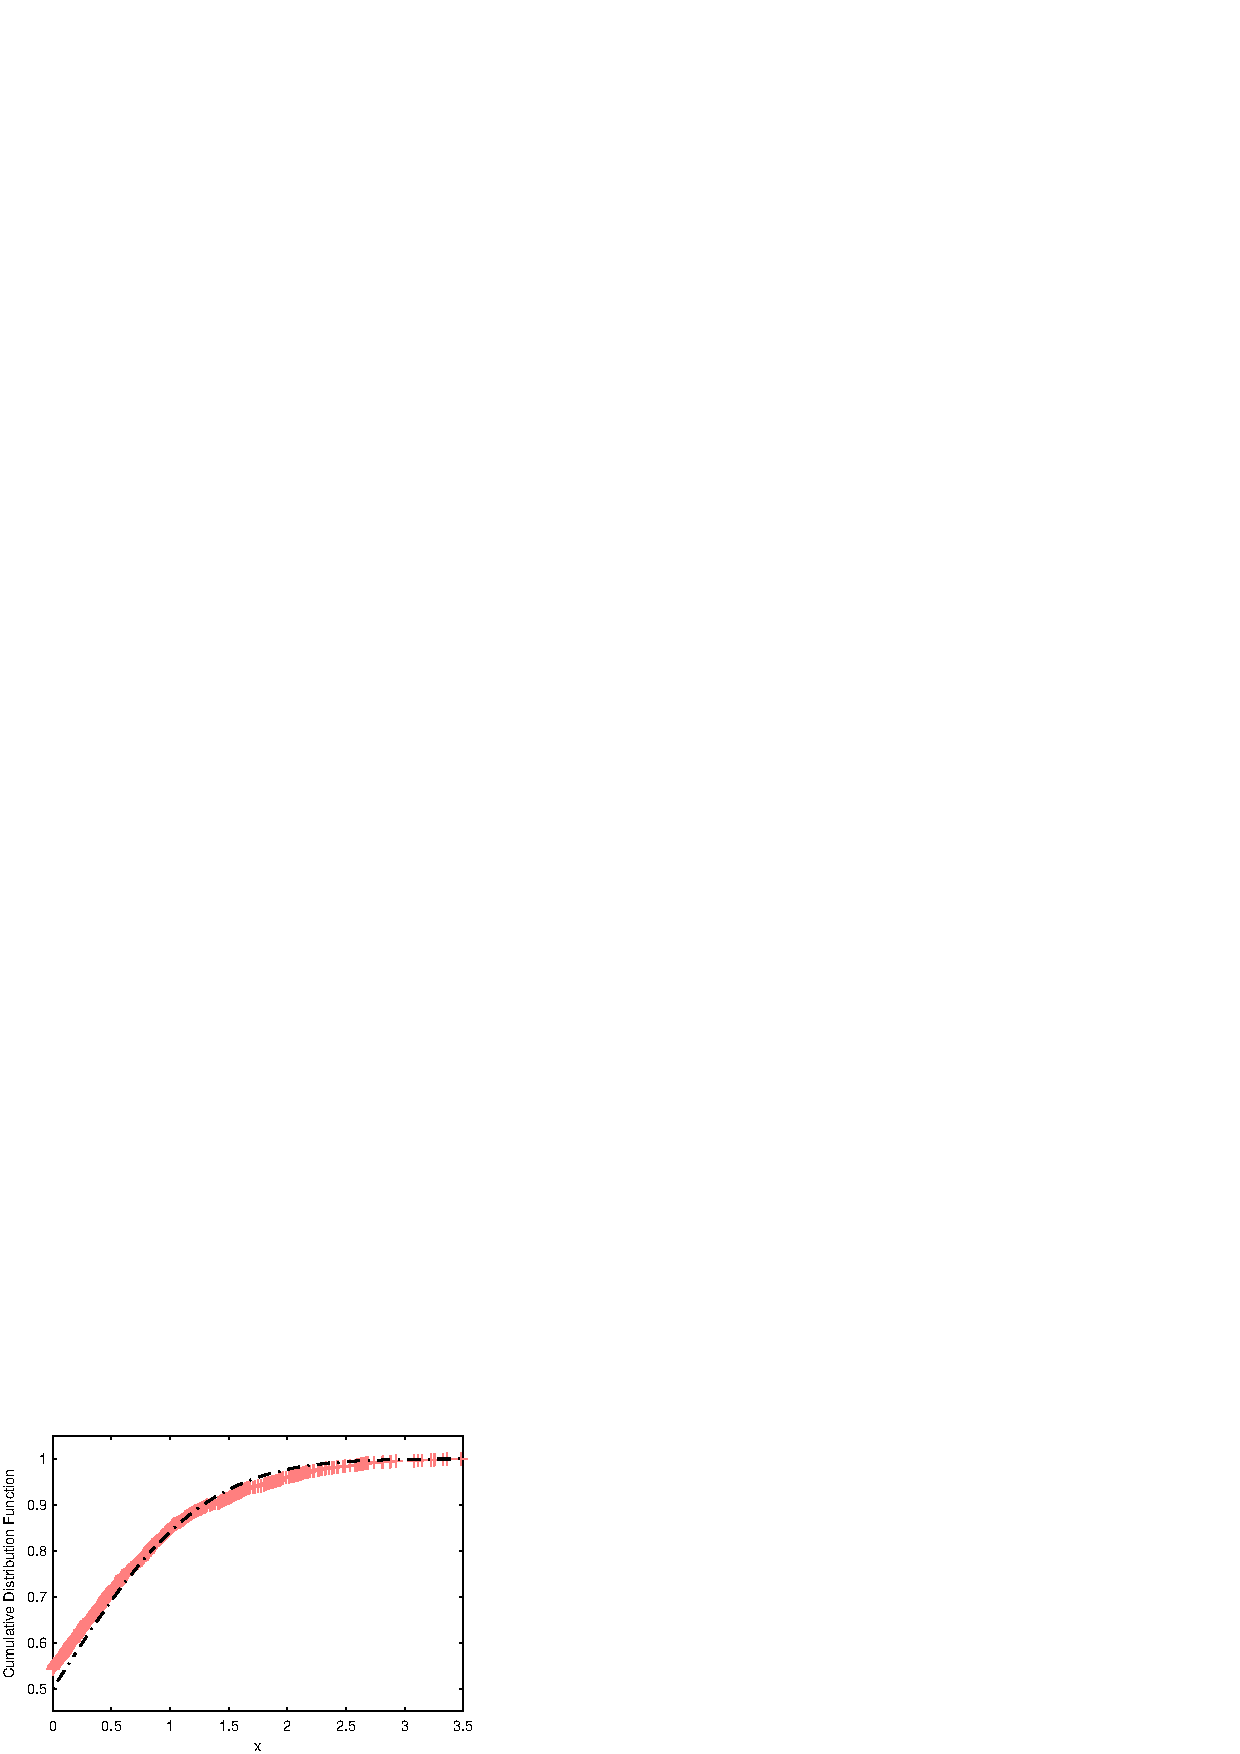
\includegraphics[width=0.4\textwidth]{methodology/selection/fig01aecdf_g}
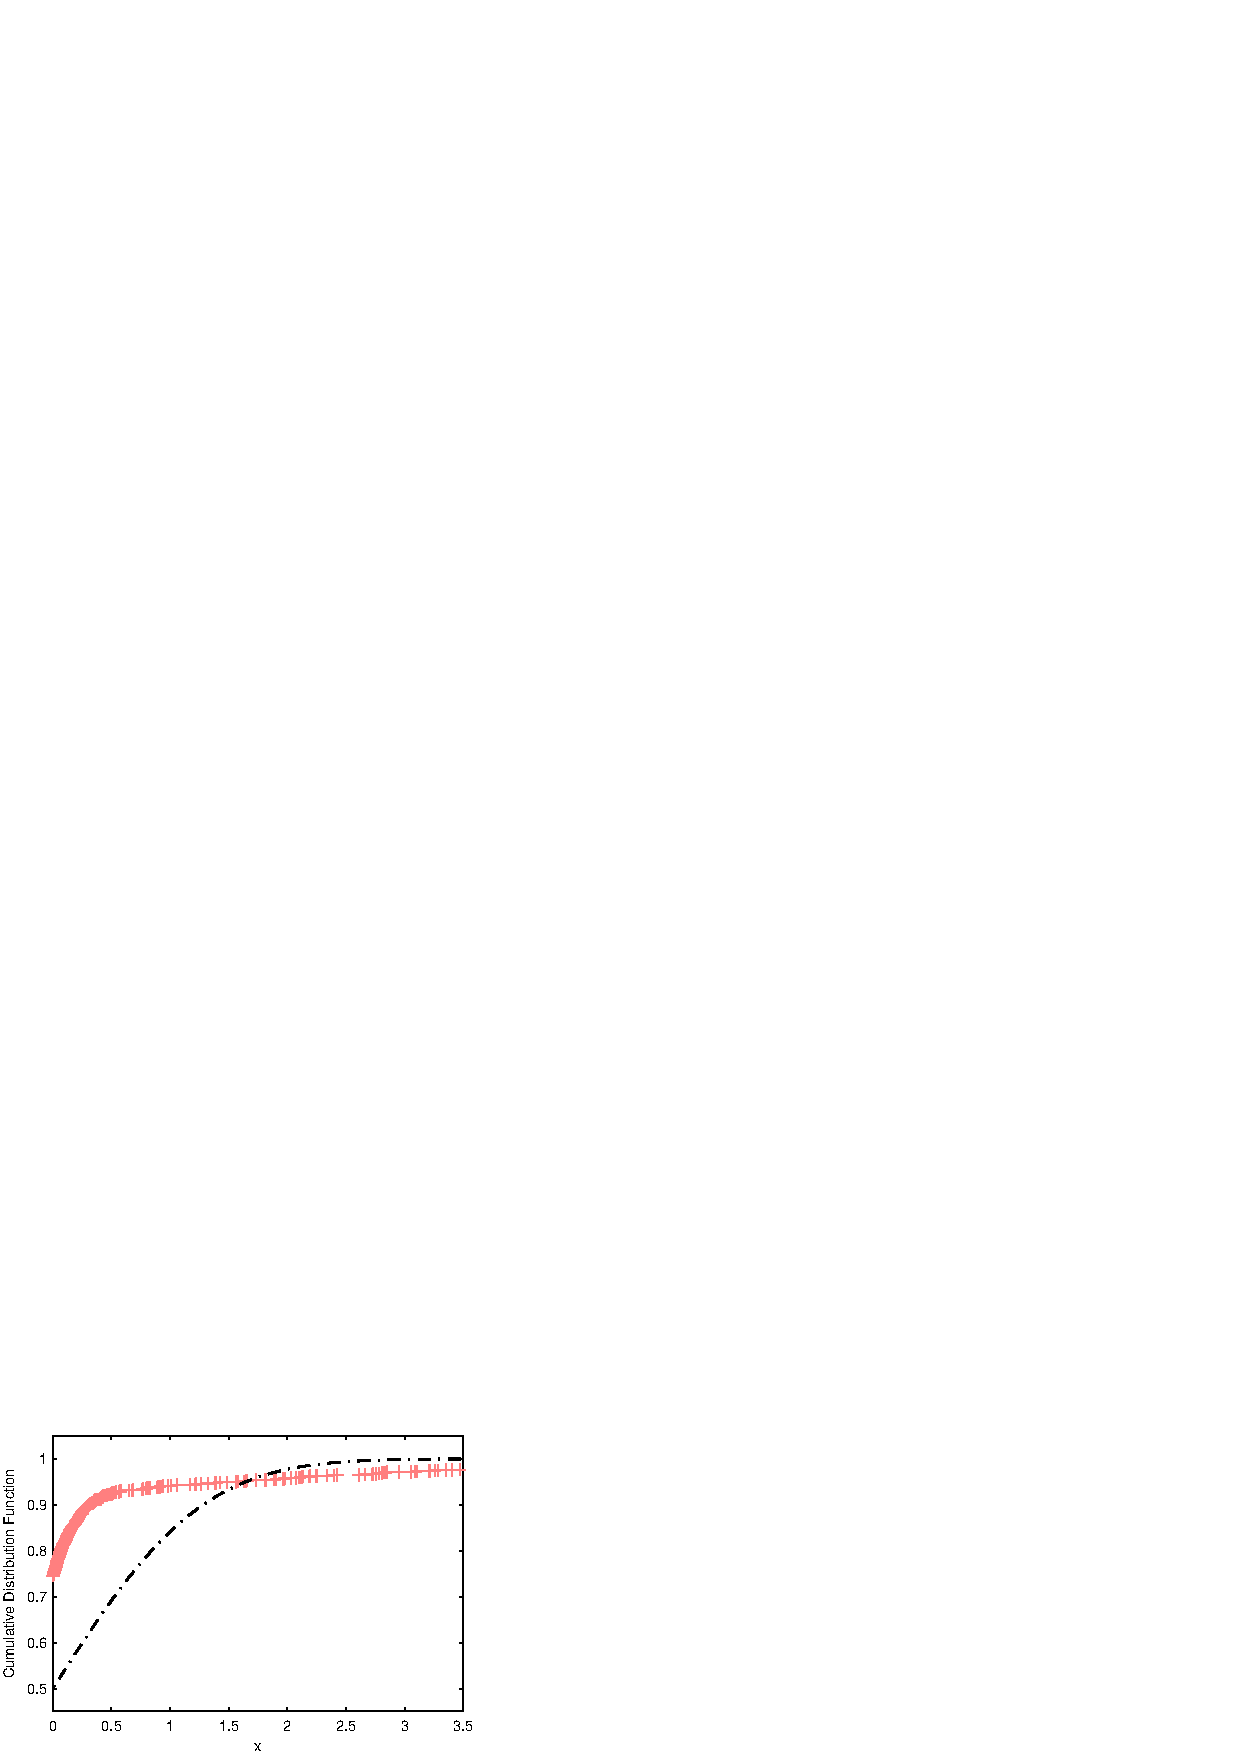
\includegraphics[width=0.4\textwidth]{methodology/selection/fig01becdf_b}
\caption{The empirical and theoretical (Gaussian) cumulative distribution functions for exemplary sub-signals from machine in good condition (left panel) and damaged one (right panel). The black dashed line represents the reference cumulative distribution function of Gaussian distribution.}\label{selection_fig1}
\end{center}
\end{figure}
The idea of using the Kolmogorov-Smirnov statistic for spikiness detection is illustrated in Fig.~\ref{selection_fig1}, where we present the empirical and theoretical cumulative distribution functions for real data set analyzed in Sec.~\ref{selection_bearing}. In the left panel of Fig.~\ref{selection_fig1} we show the cumulative distribution functions (empirical and theoretical - Gaussian) for sub-signal corresponding to the frequency $f=2325$~Hz for machine in good condition while in the right panel for the damaged one. One can observe in the left panel the analyzed functions are closer than in the right panel, therefore the $KSS$ for this frequency band has lower value for the sub-signal from machine in good condition.\\ In~\cite{Stephens1979591,Burnecki2011293} one can find more properties of the $KSS$ statistic and statistical test based on it. We only mention here the $KSS$ statistic tends to zero (almost surely) when number of elements in set $T$ tends to infinity. Moreover the distribution of $KSS$ statistic defined in (\ref{selection_K-S}) is normal. The first fact is a result of Glivenko-Cantelli theorem~\cite{Tucker1959828} while the second it is so called the distribution-free property.\\
The next statistic that might be a useful tool for informative band selection is an extension of the mentioned Kolmogorov-Smirnov. Similar to $KSS$, it is based on the distance between theoretical and empirical cumulative distribution functions for underlying sub-signal. The selector, called Anderson-Darling statistic, belongs to the Cramer-von Mises family of statistics which incorporate the idea of quadratic norm. The Cramer-von Mises statistic for frequency band $f$ is defined by~\cite{Burnecki2011293}
\begin{eqnarray}
Q(f)=\#T\int^{\infty}_{-\infty} \! \left(ECDF_{f}\left(x \right) - \Phi_f\left(x\right)\right)^2 \phi \left(x\right) \, \mathrm{d} x
\end{eqnarray}
where $\phi \left(x\right)$ is a suitable function which puts weights to the squared difference $\left(ECDF_{f}\left(x \right) - \Phi_f\left(x\right)\right)^2$. Moreover functions $ECDF_f(x)$ and $\Phi_f(x)$ are defined in (\ref{selection_FF}) and (\ref{selection_ECDF}), respectively. When $\phi(x)=1$, $Q(f)$ is called the Cramer-von Mises statistic. In this case we denote it as $CVM$. If $\phi\left(x\right)=\left[ \Phi_f\left(x\right) \left( 1-\Phi_f\left(x\right) \right) \right]^{-1}$, the above definition yields the Anderson-Darling statistic.  In the further analysis it is denoted as $AD$. Similarly to the Kolmogorov-Smirnov statistic there exist statistical tests that allow to test the proper distribution of examined data by using the $CVM$ and $AD$ statistics. More details can be found in~\cite{Anderson1952193,Anderson1954765,Burnecki2012}. The Cramer-von Mises test has better properties than the Kolmogorov-Smirnov test, but it is relatively insensitive to "tails" of the distribution. In order to eliminate this disadvantage the Anderson-Darling test was introduced. The Anderson--Darling test is a statistical test of whether a given sample of data is drawn from a given probability distribution. In our case the base distribution is normal. The test is one of the most powerful statistical tools for detecting deviations from normality.\\
\subsection{Quantile-quantile plot-based selectors}
Except of statistical tests with explicit hypothesis, there are some visual tests to compare two distributions, e.g. the theoretical distribution and the empirical one. One of the most famous examples is the quantile-quantile plot (QQplot),~\cite{Cleveland1994}. Plot of the theoretical distribution quantiles versus the underlying ones might be useful to recognize goodness-of-fit. Straight line on the QQplot means that compared distributions have the same shape. Straight line with equal scales on the axes means equal distributions. If there is no straight line, then one can compare, for example, tail heaviness of both distributions. In most of numerical packages (MATLAB, R) there is an additional straight line plotted to make analysis easier. This line connects two points: first and third quartiles of both distributions. To make this test numerical, we propose to measure the horizontal distance between the QQplot markers and the additional straight line. One can note that statistics contained in this group require sorting, similar to the previous group. Nevertheless, the lack of explicit hypothesis of gaussianity test based on the QQplot tends us to classify them into an individual group.\\
\begin{figure}[!ht]
\begin{center}
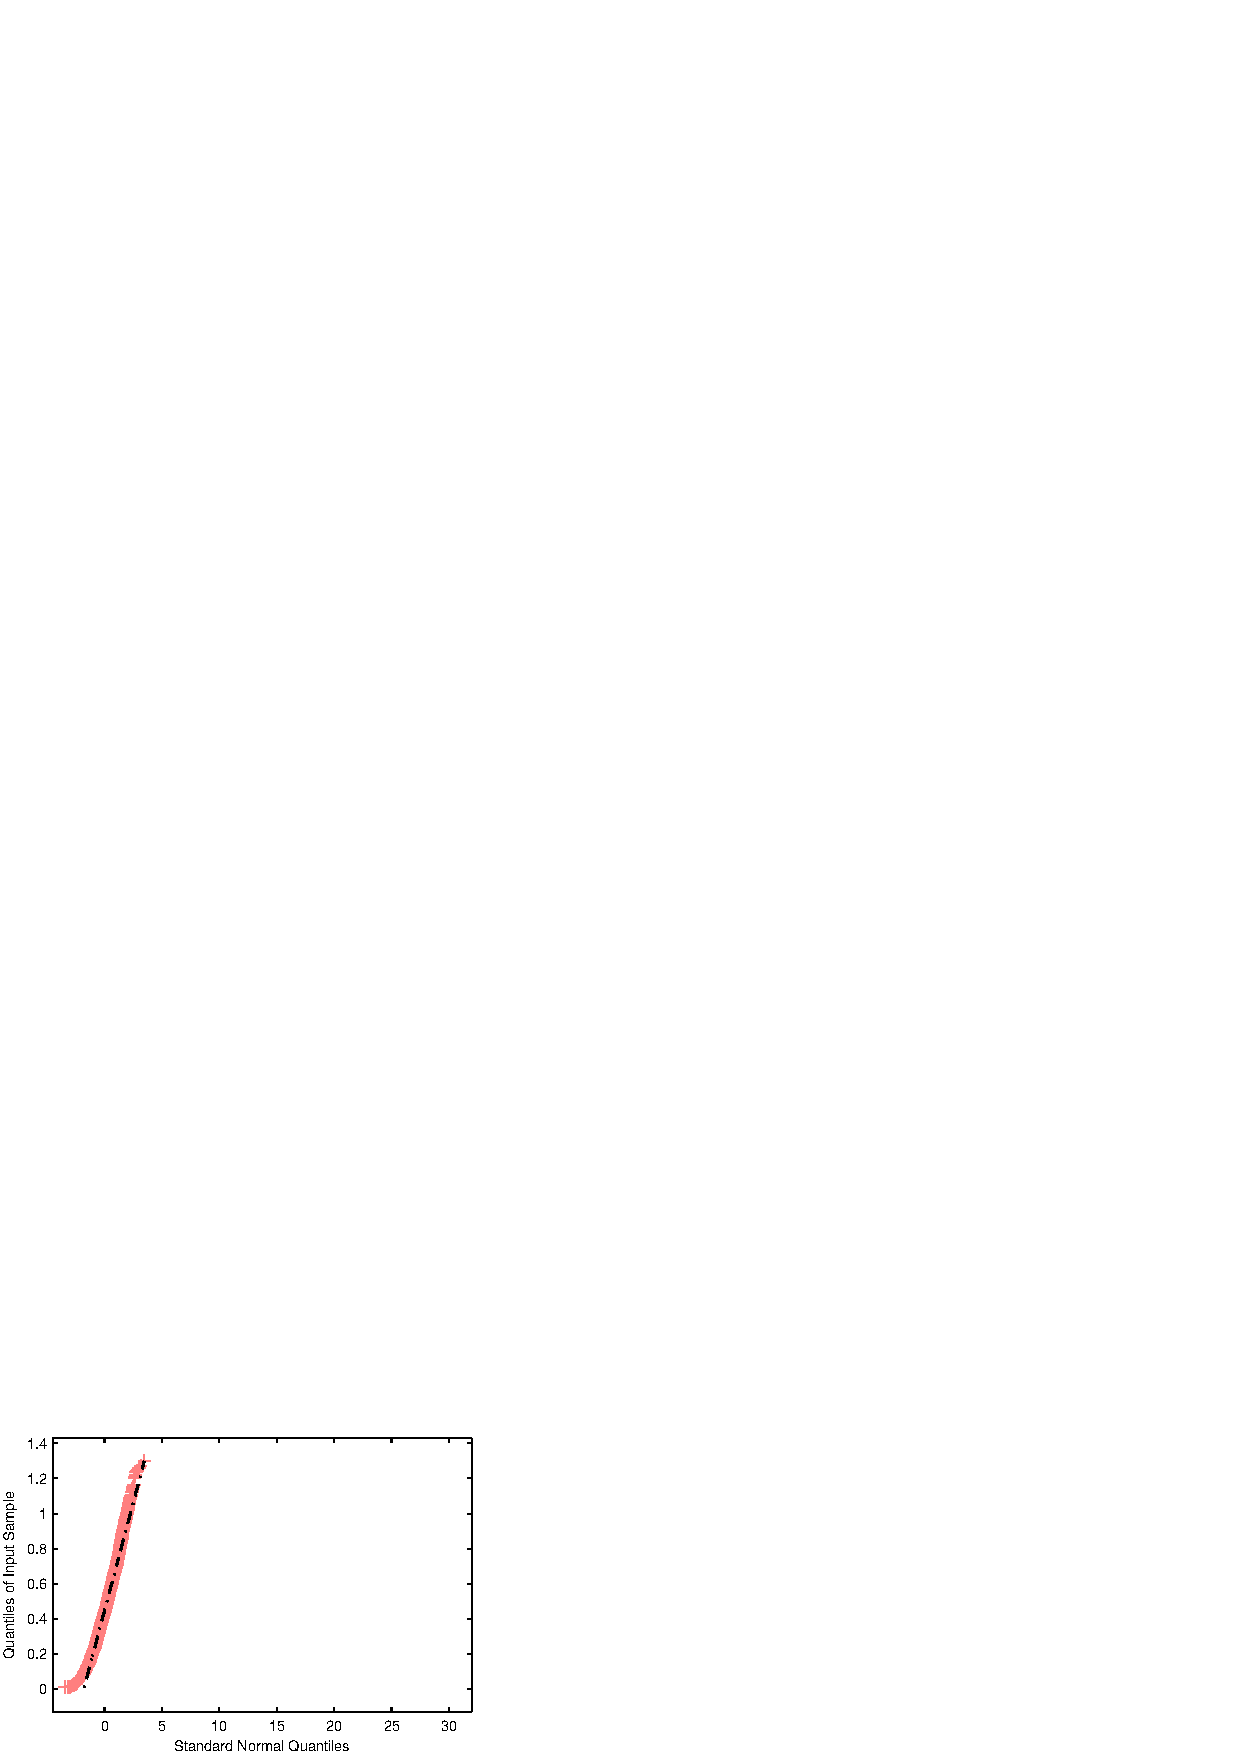
\includegraphics[width=0.4\textwidth]{methodology/selection/fig02aqqplot_g}
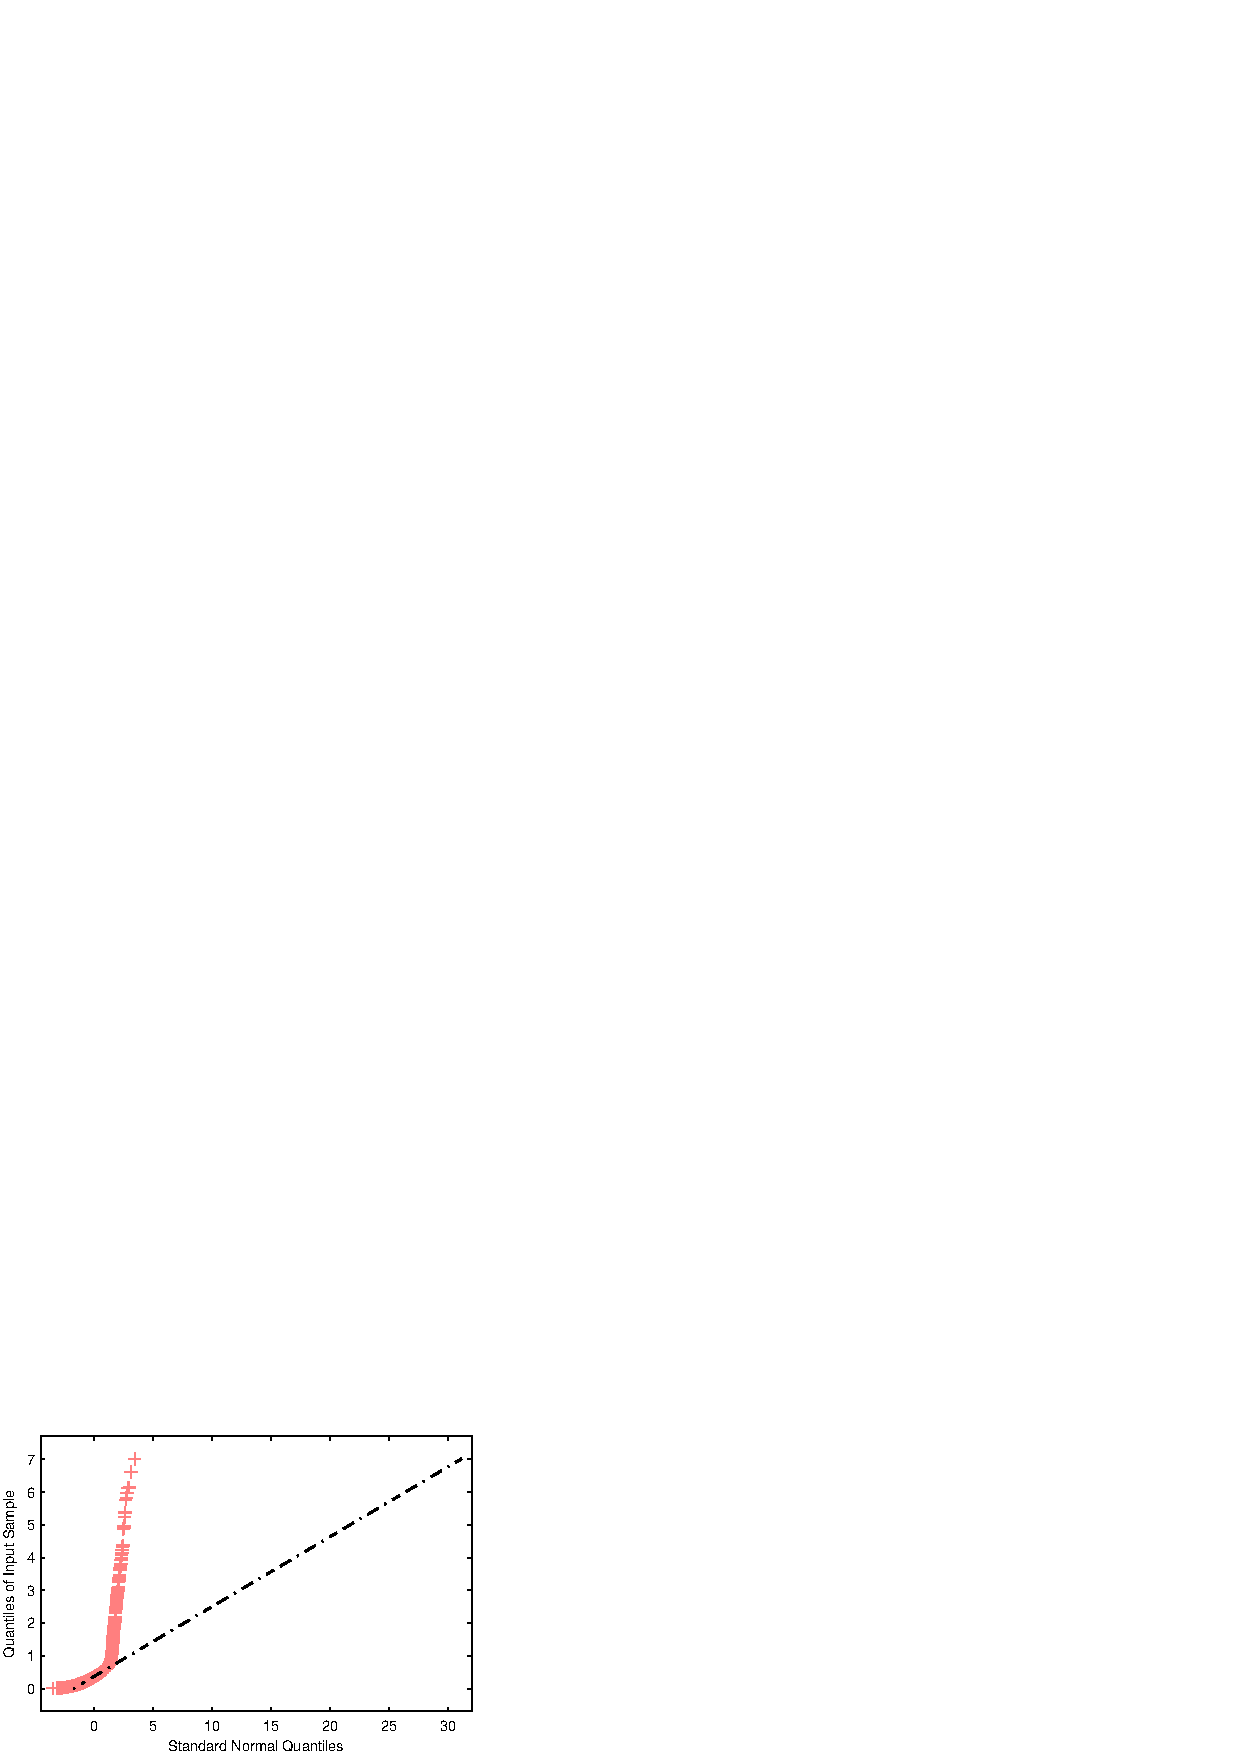
\includegraphics[width=0.4\textwidth]{methodology/selection/fig02bqqplot_b}
\caption{QQplot of the healthy (left panel) and unhealthy (right panel) sub-signal compared to the normal distribution. The black dashed line represents the reference quantile line for Gaussian distribution. Note that only horizontal distance between markers and line is quantified by $H_{aver}$ and $H_{max}$.}\label{selection_fig2}
\end{center}
\end{figure}
For this test, we propose to compute mean and maximum of those distances. The formula for the maximum distance between the Gaussian distribution and the sub-signal corresponding to the frequency band $f$ is as follows:
\begin{eqnarray}
H_{max}(f)=\max_{1\leq k \leq \#T}{ \left| \Phi^{-1}_f\left( \frac{2k-1}{2\#T} \right) - a S(k,f)-b \right| },
\end{eqnarray}
where $\Phi_f^{-1}$ is the inverse of $\Phi_f$ defined in (\ref{selection_FF}) for $\mu=0$ and $\sigma=1$, $S(k,f)$ is the $k$-th value of ascending sorted sub-signal $\{|STFT(t,f)|\}_{t\in T}$, $a=\dfrac{\Phi^{-1}(0.75)-\Phi^{-1}(0.25)}{q_{f}(0.75)-q_{f}(0.25)}$, $b=\Phi^{-1}(0.75)-aq_{f}(0.75)$ and $q_{f}(p)$ is a $p$-th order quantile of a sub-signal $\{|STFT(t,f)|\}_{t\in T}$. The formula for the average distance is analogous with the $\max$ function substituted by the arithmetic mean. We denote the corresponding statistic as $H_{aver}$. The exemplary QQplots  for real data examined in Sec.~\ref{selection_bearing} of a healthy signal (for a given frequency bin) is presented in Fig.~\ref{selection_fig2} (left panel) while for the sub-signal with defect - in the right panel of Fig.~\ref{selection_fig2}. We observe the healthy signal is closer to Gaussian distribution than the unhealthy one. Both average and maximum horizontal distances between straight line and markers are significantly larger in the right panel.
\subsection{Local maxima method-based selector}
The last procedure that allows for construction of a selector for local damage detection is based on the local maxima method~\cite{Obuchowski2014325,Obuchowski2014389}. For each frequency band (i.e. each sub-signal) we check the local maximum occurrence. We assume that local maximum occurs at a given time point when the modulus of STFT value therein is higher than the other values in its neighborhood of a length not less than a certain value - $r$. Then, for each frequency band we create a new binary vector which is a transformation of the original data into zero-one series. More precisely, we put 1 at a time point when the local maximum occurs and 0 otherwise. Let us point that the binary values obtained in this way minimize influence of insignificant signals for local damage detection as well as maximize influence of characteristic signals for locally damaged machinery. In our methodology for each time point we use the vector of weights (VoW), which is a vector of averaged maxima occurrence, i.e. VoW at point $t$ is defined as follows:
\begin{eqnarray}
W(t)=\frac{1}{\#\textit{F}}\sum_{f\in\textit{ F}}M(t,f),
\end{eqnarray}
where $M(t,f)$  represents binary valued vector of the local maxima occurrence at the time point  $t$ and frequency $f$. After multiplying each previously computed binary value by the value of VoW at the corresponding time point we obtain an enhanced spectrogram. Therefore the enhanced spectrogram at point $(t,f)$ is defined as follows:
\begin{eqnarray}
ENH(t,f)=W(t)M(t,f).
\end{eqnarray}
More details of the procedure for the enhanced spectrogram construction for different applications one can find in~\cite{Obuchowski2014325,Obuchowski2014389}. The selector based on the local maxima method for frequency band $f$ is constructed as follows:
\begin{eqnarray}
LM(f)=\frac{1}{\#T}\sum_{t\in T}ENH(t,f).
\end{eqnarray}
\FloatBarrier